\documentclass[a4paper, 12pt]{report}
\usepackage[T1]{fontenc}
\usepackage[utf8]{inputenc}
\usepackage[english]{babel}
\usepackage{mathtools}
\usepackage{amsfonts}
\usepackage{amsmath}
\usepackage{mathrsfs}
\usepackage{enumitem}
\usepackage{booktabs}
\usepackage{array}
% Avoid paragraph indent
\setlength{\parindent}{0pt}
% Useful floor and ceiling functions
\DeclarePairedDelimiter{\floor}{\lfloor}{\rfloor}
\DeclarePairedDelimiter{\ceil}{\lceil}{\rceil}
% Argmax/Argmin notation
\DeclareMathOperator*{\argmax}{argmax} 
\DeclareMathOperator*{\argmin}{argmin}
% Modified margins
\usepackage[margin=2cm]{geometry}
% This avoids hypenation
\hyphenpenalty=10000
\usepackage{tikz}
\usetikzlibrary{arrows,calc,positioning,shadows,shapes}
\usepackage{graphicx}
\usepackage{subfig}
\captionsetup[figure]{labelfont={bf},name={Figure},labelsep=period}
\captionsetup[table]{labelfont={bf},name={Table},labelsep=period}

\usepackage{float}


\begin{document}
	
\title{Digital Communications and Laboratory \\ Third Homework}
\author{Faccin Dario, Santi Giovanni}
\date{}
\maketitle


\section*{PROBLEM}
The following system was considered. A stream of QPSK symbols is upsampled with period T/4 and filtered with a filter $q_c$ which output is $s_c\left(n\frac{T}{4}\right)= \alpha s_c\left((n-1)\frac{T}{4}\right)+\beta a_{n-5}'$. This signal is transmitted through the channel, which introduces the noise component $w_c\left(n\frac{T}{4}\right)$ with PSD $\mathcal{P}_{w_c}(f) = N_0$. Note that noise components are iid with \textit{pmd} $\sim \mathcal{CN}(0,\sigma_{w_c}^2)$. The SNR at the output of the system is therefore 
\begin{equation*}
\Gamma = \frac{M_{s_c}}{N_0\frac{1}{T}} = \frac{\sigma^2_a E_{q_c}}{\sigma_{w_c}^2}
\end{equation*}
with $\sigma^2_a=2$ and $E_{q_c} = \sum_m | q_c \left(m\frac{T}{4}\right) |^2$.

\begin{figure}[H]
	\centering
	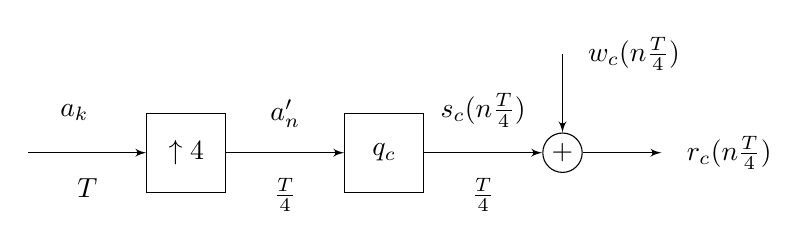
\begin{tikzpicture}[auto,>=latex']
	\tikzstyle{block} = [draw, rectangle, minimum height=1cm, minimum width=1cm]
	
	\node [coordinate, label={[label distance=0.4cm]45:$a_k$}] (start) {};
	\node [block, right = 1.5cm of start] (intpl){$\uparrow 4$};
	\node [coordinate, label={[label distance=0.2cm]90:$a'_n$}, right = 0.75 cm of intpl] (c1) {};
	\node [block, right = 1.5cm of intpl] (imp){$q_c$};
	\node [draw, circle,minimum size=0.5cm,inner sep=0pt, right = 1.5cm of imp] (sum){$+$};
	\node [coordinate, label={[label distance=0.2cm]90:$s_c(n \frac{T}{4})$}, right = 0.75cm of imp] (c2) {};
	
	\node [coordinate, label={[label distance=0.2cm]0:$w_c(n \frac{T}{4})$}, above = 1cm of sum] (wgn) {};
	\node [coordinate, label={[label distance=0.2cm]0:$r_c(n \frac{T}{4})$}, right = 1cm of sum] (end) {};
	
	\draw [->] (start) --node[label={[label distance=0.2cm]270:$T$}]{} (intpl);
	\draw [->] (intpl) --node[label={[label distance=0.2cm]270:$\frac{T}{4}$}]{} (imp);
	\draw [->] (imp) --node[label={[label distance=0.2cm]270:$\frac{T}{4}$}]{} (sum);
	\draw [->] (wgn) --node[]{} (sum);
	\draw [->] (sum) --node[]{} (end);
	
	\end{tikzpicture}
	\caption{Model for the transmission system of Problem 1.}
	\label{Model_1} 
\end{figure}

The QPSK symbols are generated with a PN sequence of length $L=2^{20}-1$ in order to provide a stream of bits with spectral characteristics similar to those of a white noise signal. Two consecutive bits are then coupled and mapped into one of the possible constellations symbols, associating the first and second bit to the real and imaginary part respectively. \\
The $q_c$ filter in linear and frequency domain is given in Figures [\ref{qc}].

\begin{figure}[H]
	\centering
	\subfloat{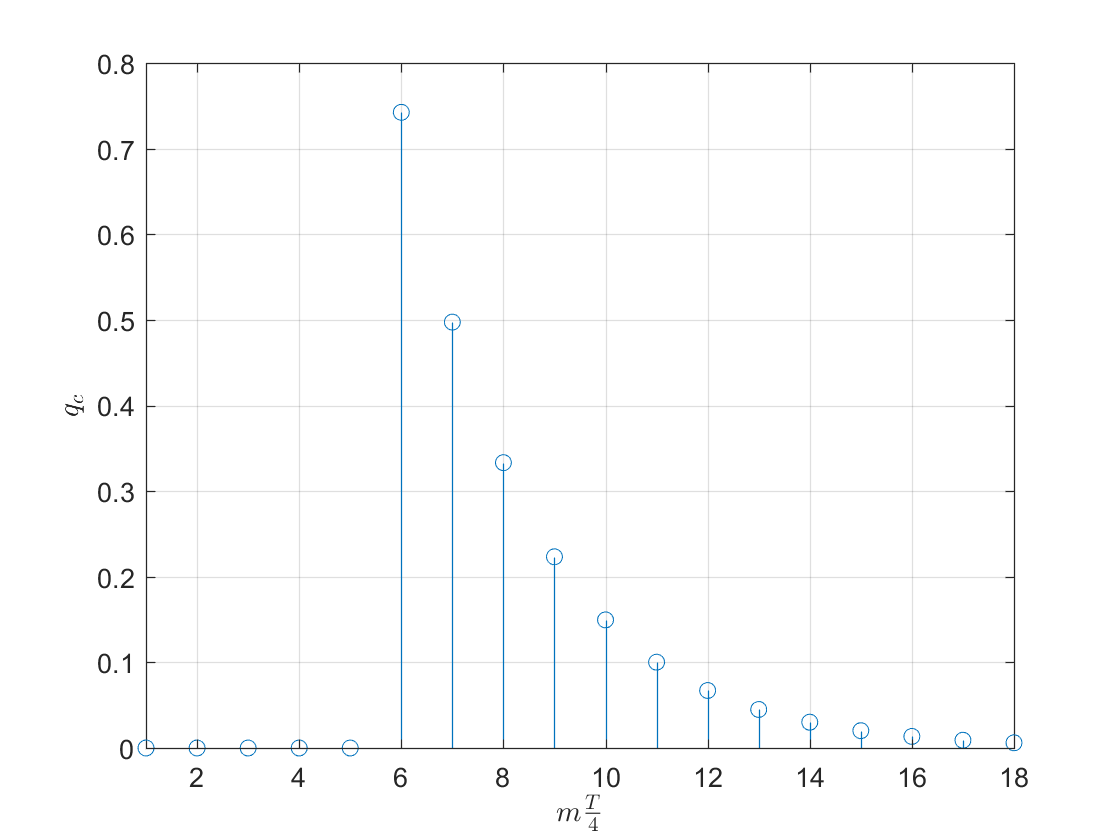
\includegraphics[width=9cm]{images/qc}}
	\subfloat{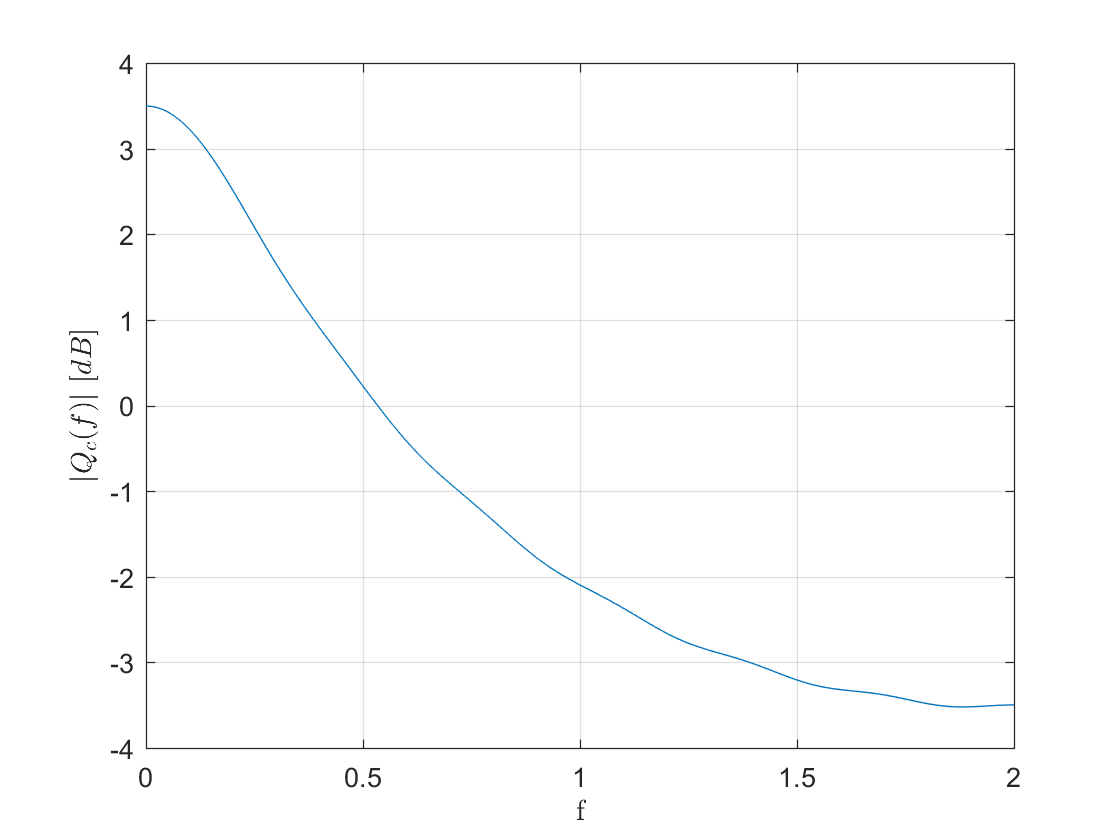
\includegraphics[width=9cm]{images/Qc_f}}
	\caption{Impulse response (left) and Frequency response (right) of the filter $q_c$.}\label{qc}
\end{figure}

In the following, 6 different receiver configurations are studied. For each of this, an SNR value of $\Gamma = 10$ $dB$ was assumed.


\clearpage
\subsection*{Receiver a}
\begin{figure}[H]
	\centering
	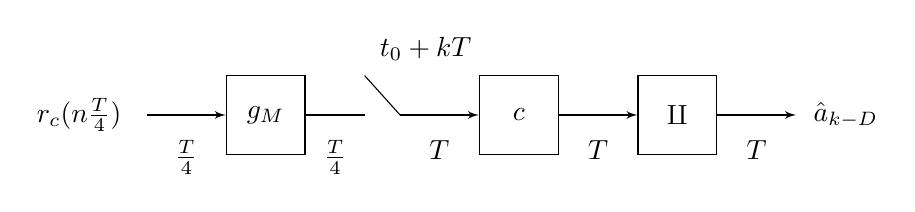
\begin{tikzpicture}[auto,>=latex']
	\tikzstyle{block} = [draw, rectangle, minimum height=1cm, minimum width=1cm]
	
	\node [coordinate, label={[label distance=0.2cm]180:$r_c(n \frac{T}{4})$}] (start) {};
	\node [block, right = 1cm of start] (matchedf){$g_M$};
	\node [coordinate, right = 0.75 cm of matchedf] (c0) {};
	\node [coordinate, above = 0.5 cm of c0, label={[label distance=0.1cm]45:$t_0 + kT$} ] (c1) {};
	
	\node [coordinate, right = 1.2cm of matchedf] (c2) {};
	
	\node [block, right = 1cm of c2] (cfilter){$c$};
	\node [block, right = 1cm of cfilter] (detector){$\amalg$};
	
	\node [coordinate, right = 1cm of detector, label={[label distance=0.1cm]0:$\hat{a}_{k-D}$}] (end){};
	
	\draw [->] (start) --node[label={[label distance=0.2cm]270:$\frac{T}{4}$}]{} (matchedf);
	\draw [-] (matchedf) --node[label={[label distance=0.2cm]270:$\frac{T}{4}$}]{} (c0);
	\draw [-] (c1) --node[]{} (c2);
	\draw [->] (c2) --node[label={[label distance=0.2cm]270:$T$}]{} (cfilter);
	\draw [->] (cfilter) --node[label={[label distance=0.2cm]270:$T$}]{} (detector);
	\draw [->] (detector) --node[label={[label distance=0.2cm]270:$T$}]{} (end);
	
	\end{tikzpicture}
	\caption{Model for the receiver (a).}
	\label{Receiver_a} 
\end{figure}

The receiver filter consists of a filter $g_M$ matched to the transmission filter $q_c$. From now on, we may refer to the global impulse response of the system at the input of the \textit{linear equalizer} $c$ as $h = g_c * g_M$. Since it is defined @$\frac{T}{4}$, a downsampling of a factor 4 is required between the output of $h$ and the input of $c$. \\
The filter $c$ attempts to find the optimum trade-off between removing the ISI and enhancing the noise at the decision point. Since the LE can be seen as a particular case of a DFE, we evaluated the coefficients of the filters $c$ and $b$ (will be introduced from Receiver (b)) using the same algorithm which exploits the Wiener filter theory to determine the optimum coefficients. \\
Let the filter $c$ and $b$ have length $M_1$ and $M_2$, with a delay $D$ introduced by $c$. Then the LE can be seen as a DFE with $M_2=0$. The coefficients are computed using the MSE applied to the cost function
\begin{equation}
J = E \left[|a_{k-D}-y_k|^2\right]
\end{equation}
The optimum FF filter is given by
\begin{equation*}
\mathbf{c}_{opt} = \mathbf{R}^{-1}\mathbf{p}
\end{equation*}
where the matrices $\mathbf{R}$ and $\mathbf{p}$ are computed using
\begin{equation}
\mathbf{[R]}_{p,q} = \sigma_a^2 \left( \sum_{j=-N_1}^{N_2}h_jh^*_{j-(p-q)}-\sum_{j=1}^{M_2}h_{j+D-q}h^*_{j+d-p} \right) + r_{\tilde{w}}(p-q)
\end{equation}
\begin{equation}
\mathbf{[p]}_p = \sigma_a^2 h^*_{D-p}, \quad\quad\quad\quad\quad\quad\quad\quad\quad\quad\quad p,q = 0,1,\dots,M_1-1
\end{equation}
The optimum FB coefficients are given by
\begin{equation}
b_i = -\sum_{l=0}^{M_1-1}c_{opt,l}h_{i+D-l} \quad\quad\quad\quad\quad\quad\quad\quad\quad\quad\quad i =1,2,\dots,M_2
\end{equation}

The minimum-cost function can be expressed in close form as:
\begin{equation}
J_{min} = \sigma^2_a \left( 1-\sum_{l=0}^{M_1-1} c_{opt,l}h_{D-l}\right)
\end{equation}

The output signal is 
\begin{equation}
\begin{split}
y_k &= x_{FF,k} + x_{FB,k} \\
	&= \sum_{i=0}^{M_1-1}c_ix_{k-i} + \sum_{j=1}^{M_2}b_ja_{k-D-j}
\end{split}
\end{equation}

The equalizing filter $c$ and the overall impulse response $\psi_i=h*c_i$ for an SNR of $\Gamma = 10$ dB are given in Figure [\ref{filters_a}]. 

\begin{figure}[H]
	\centering
	\subfloat{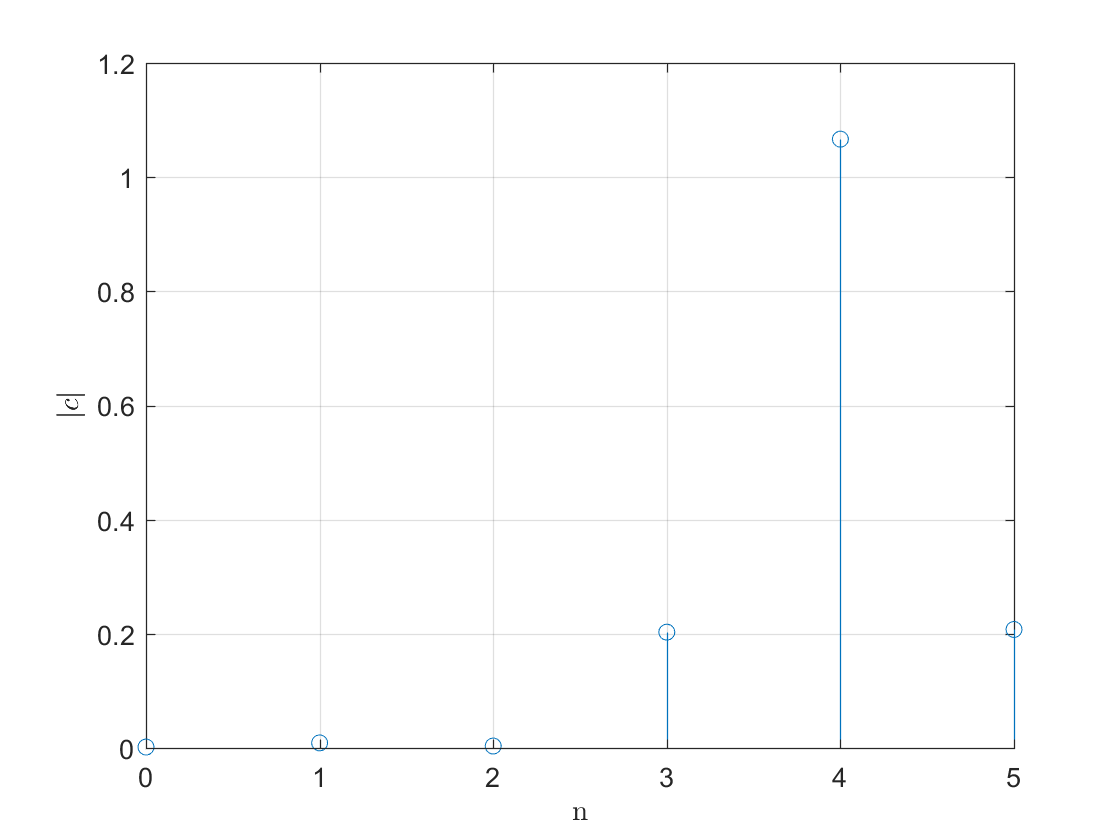
\includegraphics[width=9cm]{images/RecA_c}}
	\subfloat{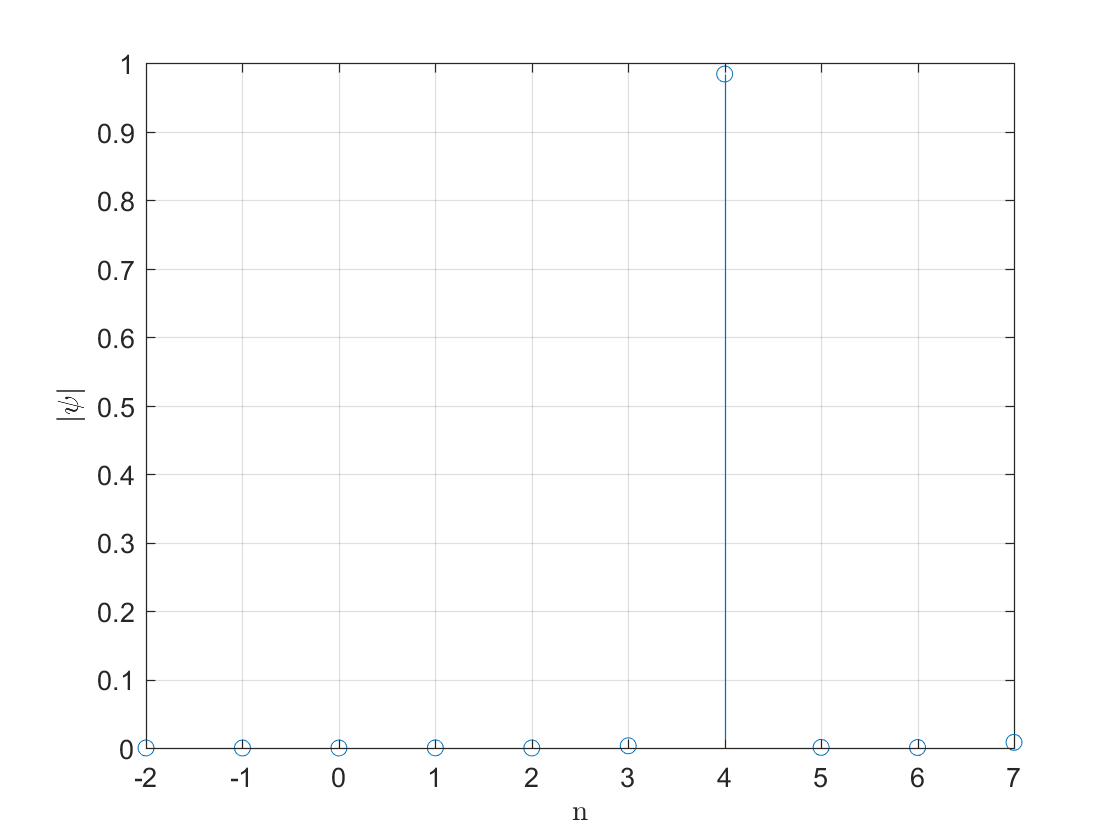
\includegraphics[width=9cm]{images/RecA_psi}}
	\caption{Coefficients of the Equalizer filter $c$ (left) and of the overall impulse response $\psi_i$ (right).}\label{filters_a}
\end{figure}

The parameters we obtained are reported in Table [\ref{Tab_a}].

\begin{table}[H]
	\centering
	\begin{tabular}{c c c c}
		\toprule
		$\mathbf{\bar{t}_0}$ & $\mathbf{M_1}$ & $\mathbf{M_2}$ & \textbf{D}     \\
		\midrule
		1 & 1 & 1 & 1 \\
		\bottomrule			
	\end{tabular}
	\caption{Parameters of the Receiver (a).}
	\label{Tab_a}
\end{table}

The final signal at the output of the equalizer filter is processed by a threshold detector, which maps each received symbol according to the following rule:

\begin{equation*}
\tilde{a}_k \mapsto \hat{a}_k = \text{sgn}(\Re[\tilde{a}_k ]) +i \cdot \text{sgn}(\Im[\tilde{a}_k ])
\end{equation*}
 
Note that the actual transmitted symbol at time $k$ is detected at time $k+D$ because of the delay introduced by the filter $c$. This detection configuration will be used also for receivers $b$, $c$ and $d$. 

\clearpage
\subsection*{Receiver b}
The only difference with Receiver (a) is that here the \textit{Decision Filter Equalizer} introduces a feedback filter to remove the postcursors of the impulse response $h$ at the input of the FF filter. Using the algorithm described in the previous section, we obtained the filters given as follow.

\begin{figure}[H]
	\centering
	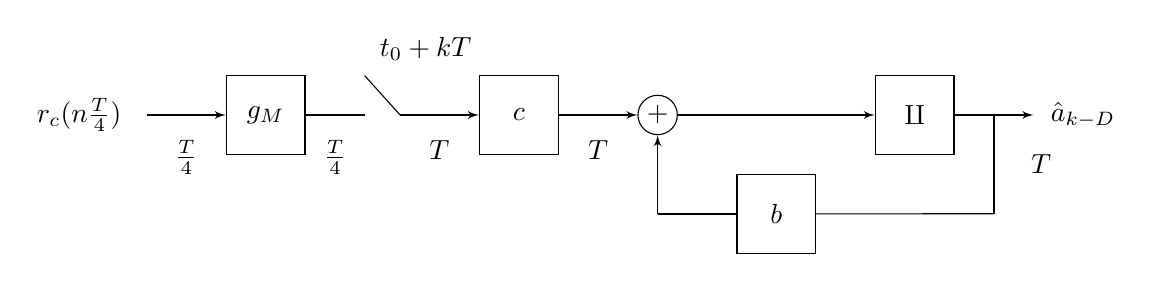
\begin{tikzpicture}[auto,>=latex']
	\tikzstyle{block} = [draw, rectangle, minimum height=1cm, minimum width=1cm]
	
	\node [coordinate, label={[label distance=0.2cm]180:$r_c(n \frac{T}{4})$}] (start) {};
	\node [block, right = 1cm of start] (matchedf){$g_M$};
	\node [coordinate, right = 0.75 cm of matchedf] (c0) {};
	\node [coordinate, above = 0.5 cm of c0, label={[label distance=0.1cm]45:$t_0 + kT$} ] (c1) {};
	
	\node [coordinate, right = 1.2cm of matchedf] (c2) {};
	
	\node [block, right = 1cm of c2] (cfilter){$c$};
	
	\node [draw, circle,minimum size=0.5cm,inner sep=0pt, right = 1cm of cfilter] (sum){$+$};
	
	\node [coordinate, below = 1cm of sum] (c3) {};	
	
	\node [block, right = 2.5cm of sum] (detector){$\amalg$};
	
	\node [coordinate, right = 0.5cm of detector] (cfin) {};
	
	\node [coordinate, below = 1.254cm of cfin] (c6) {};
	
	\node [block, right = 1cm of c3] (b){$b$};	
	
	\node [coordinate, right = 1cm of detector, label={[label distance=0.1cm]0:$\hat{a}_{k-D}$}] (end){};
	
	\draw [->] (start) --node[label={[label distance=0.2cm]270:$\frac{T}{4}$}]{} (matchedf);
	\draw [-] (matchedf) --node[label={[label distance=0.2cm]270:$\frac{T}{4}$}]{} (c0);
	\draw [-] (c1) --node[]{} (c2);
	\draw [->] (c2) --node[label={[label distance=0.2cm]270:$T$}]{} (cfilter);
	\draw [->] (cfilter) --node[label={[label distance=0.2cm]270:$T$}]{} (sum);
	\draw [->] (c3) --node[]{} (sum);
	\draw [-] (b) --node[]{} (c3);
	\draw [-] (c6) --node[]{} (b);
	\draw [-] (cfin) --node[label={[label distance=0.1cm]0:$T$}]{} (c6);
	\draw [->] (sum) --node[]{} (detector);
	\draw [->] (detector) --node[]{} (end);
	\end{tikzpicture}
	\caption{Model for the receiver (b).}
	\label{Receiver_b} 
\end{figure}

\begin{figure}[H]
	\centering
	\subfloat{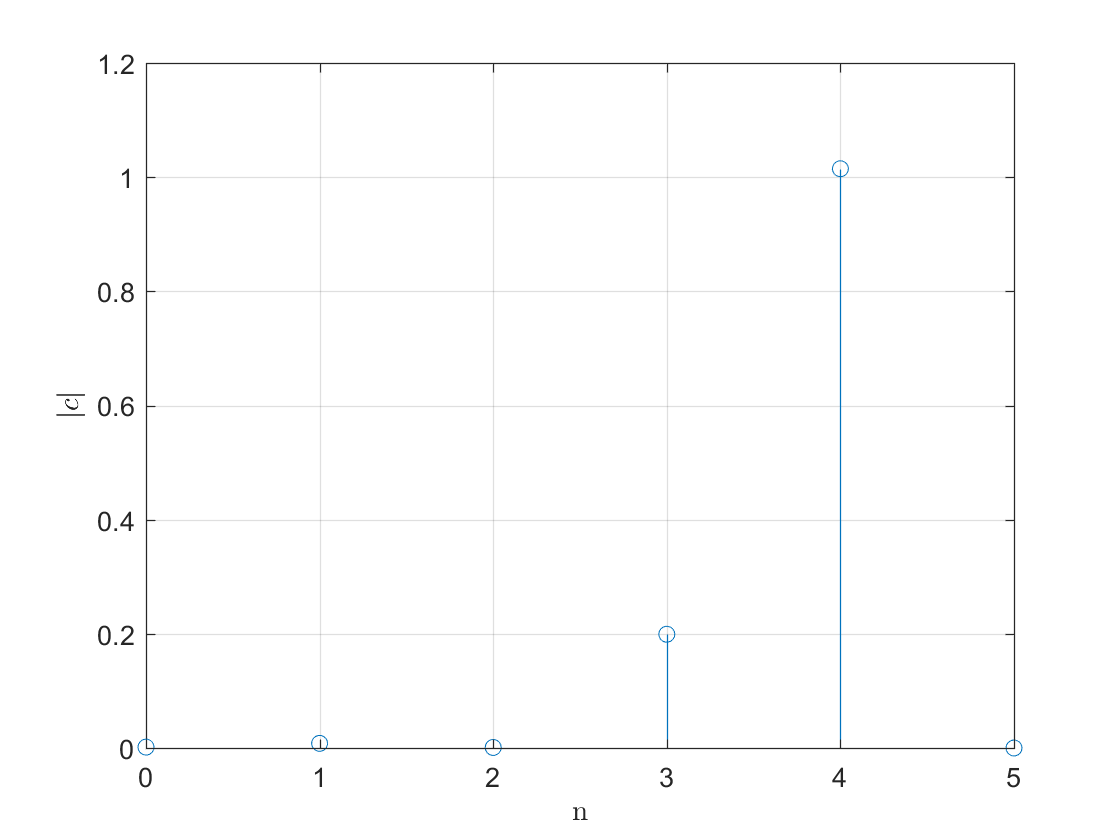
\includegraphics[width=9cm]{images/RecB_c}}
	\subfloat{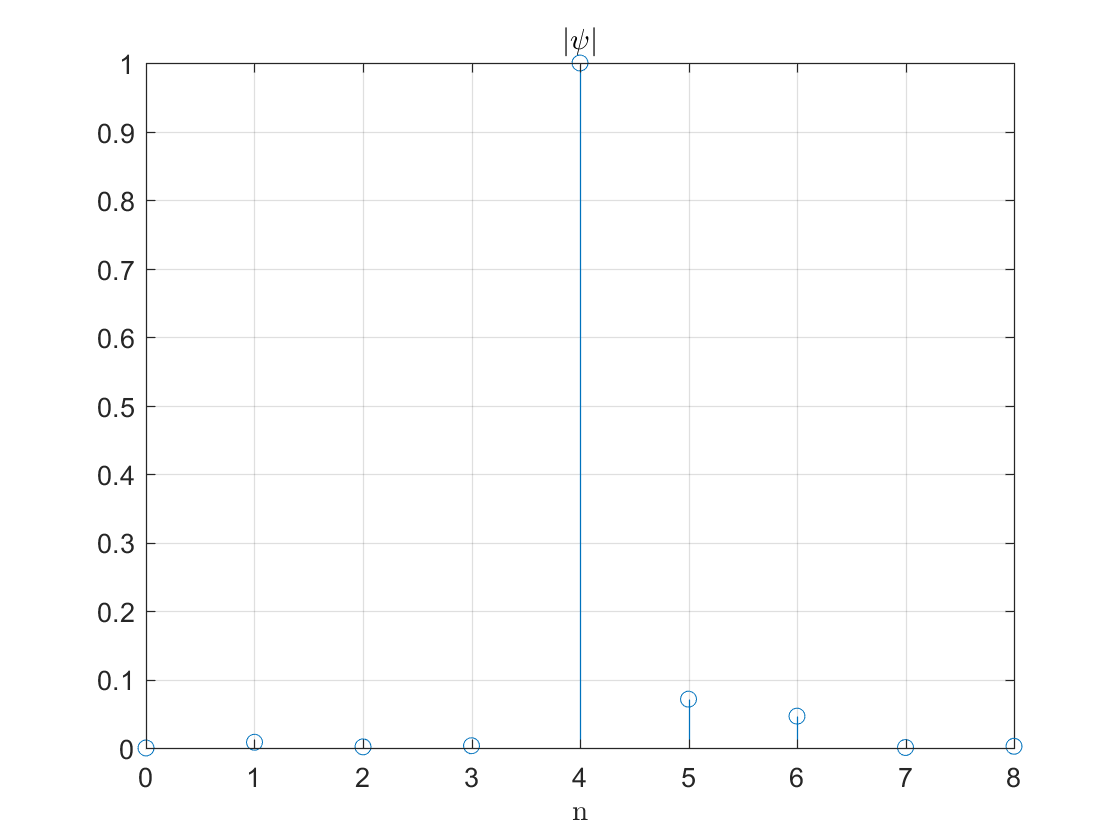
\includegraphics[width=9cm]{images/RecB_psi}}\quad
	\subfloat{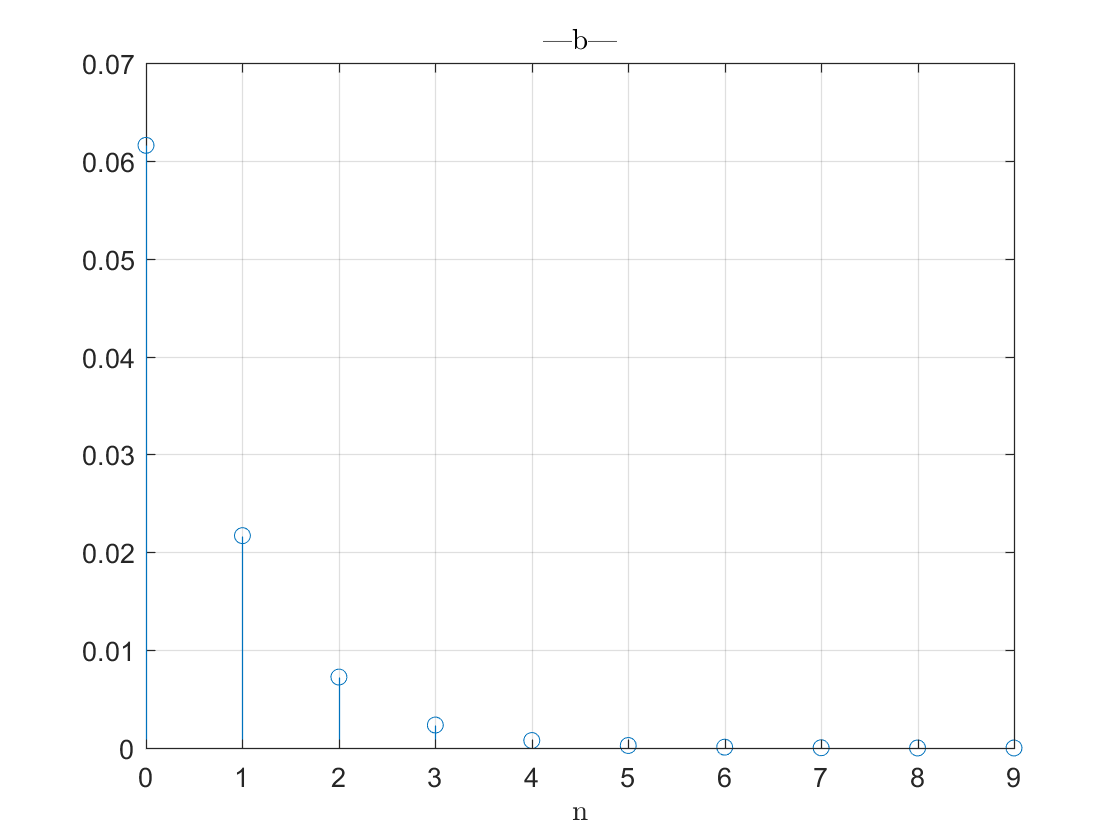
\includegraphics[width=9cm]{images/RecB_b}}
	\caption{Coefficients of the Equalizer filter $c$ (left) and of the overall impulse response $\psi_i$ (right).}\label{filters_b}
\end{figure}
\clearpage
\subsection*{Receiver c}

\begin{figure}[H]
	\centering
	\begin{tikzpicture}[auto,>=latex']
	\tikzstyle{block} = [draw, rectangle, minimum height=1cm, minimum width=1cm]
	
	\node [coordinate, label={[label distance=0.2cm]180:$r_c(n \frac{T}{4})$}] (start) {};
	\node [block, right = 1cm of start] (gaa){$g_{AA}$};
	\node [coordinate, right = 0.75 cm of gaa] (c0) {};
	\node [coordinate, above = 0.5 cm of c0, label={[label distance=0.1cm]45:$t_0 + m \frac{T}{2}$} ] (c1) {};
	
	\node [coordinate, right = 1.2cm of gaa] (c2) {};
	
	\node [block, right = 1cm of c2] (gm){$g_M$};
	
	\node [block, right = 1cm of gm] (cfilter){$c$};
	
	\node [draw, circle,minimum size=0.5cm,inner sep=0pt, right = 1cm of cfilter] (sum){$+$};
	
	\node [coordinate, below = 1cm of sum] (c3) {};	
	
	\node [block, right = 2.5cm of sum] (detector){$\amalg$};
	
	\node [coordinate, right = 0.5cm of detector] (cfin) {};
	
	\node [coordinate, below = 1.254cm of cfin] (c6) {};
	
	\node [block, right = 1cm of c3] (b){$b$};	
	
	\node [coordinate, right = 1cm of detector, label={[label distance=0.1cm]0:$\hat{a}_{k-D}$}] (end){};
	
	\draw [->] (start) --node[label={[label distance=0.2cm]270:$\frac{T}{4}$}]{} (gaa);
	\draw [-] (gaa) --node[label={[label distance=0.2cm]270:$\frac{T}{4}$}]{} (c0);
	\draw [-] (c1) --node[]{} (c2);
	\draw [->] (c2) --node[label={[label distance=0.2cm]270:$\frac{T}{2}$}]{} (gm);
	\draw [->] (gm) --node[label={[label distance=0.2cm]270:$\frac{T}{2}$}]{} (cfilter);
	\draw [->] (cfilter) --node[label={[label distance=0.2cm]270:$T$}]{} (sum);
	\draw [->] (c3) --node[]{} (sum);
	\draw [-] (b) --node[]{} (c3);
	\draw [-] (c6) --node[]{} (b);
	\draw [-] (cfin) --node[label={[label distance=0.1cm]0:$T$}]{} (c6);
	\draw [->] (sum) --node[]{} (detector);
	\draw [->] (detector) --node[]{} (end);
	\end{tikzpicture}
	\caption{Model for the receiver (c).}
	\label{Receiver_c} 
\end{figure}

\clearpage
\subsection*{Receiver d}

\begin{figure}[H]
	\centering
	\begin{tikzpicture}[auto,>=latex']
	\tikzstyle{block} = [draw, rectangle, minimum height=1cm, minimum width=1cm]
	
	\node [coordinate, label={[label distance=0.2cm]180:$r_c(n \frac{T}{4})$}] (start) {};
	\node [block, right = 1cm of start] (gaa){$g_{AA}$};
	\node [coordinate, right = 0.75 cm of gaa] (c0) {};
	\node [coordinate, above = 0.5 cm of c0, label={[label distance=0.1cm]45:$t_0 + m \frac{T}{2}$} ] (c1) {};
	
	\node [coordinate, right = 1.2cm of gaa] (c2) {};
	
	\node [block, right = 1cm of c2] (cfilter){$c$};
	
	\node [draw, circle,minimum size=0.5cm,inner sep=0pt, right = 1cm of cfilter] (sum){$+$};
	
	\node [coordinate, below = 1cm of sum] (c3) {};	
	
	\node [block, right = 2.5cm of sum] (detector){$\amalg$};
	
	\node [coordinate, right = 0.5cm of detector] (cfin) {};
	
	\node [coordinate, below = 1.254cm of cfin] (c6) {};
	
	\node [block, right = 1cm of c3] (b){$b$};	
	
	\node [coordinate, right = 1cm of detector, label={[label distance=0.1cm]0:$\hat{a}_{k-D}$}] (end){};
	
	\draw [->] (start) --node[label={[label distance=0.2cm]270:$\frac{T}{4}$}]{} (gaa);
	\draw [-] (gaa) --node[label={[label distance=0.2cm]270:$\frac{T}{4}$}]{} (c0);
	\draw [-] (c1) --node[]{} (c2);
	\draw [->] (c2) --node[label={[label distance=0.2cm]270:$\frac{T}{2}$}]{} (cfilter);
	\draw [->] (cfilter) --node[label={[label distance=0.2cm]270:$T$}]{} (sum);
	\draw [->] (c3) --node[]{} (sum);
	\draw [-] (b) --node[]{} (c3);
	\draw [-] (c6) --node[]{} (b);
	\draw [-] (cfin) --node[label={[label distance=0.1cm]0:$T$}]{} (c6);
	\draw [->] (sum) --node[]{} (detector);
	\draw [->] (detector) --node[]{} (end);
	\end{tikzpicture}
	\caption{Model for the receiver (d).}
	\label{Receiver_d} 
\end{figure}

\clearpage
\subsection*{Receiver e}

\begin{figure}[H]
	\centering
	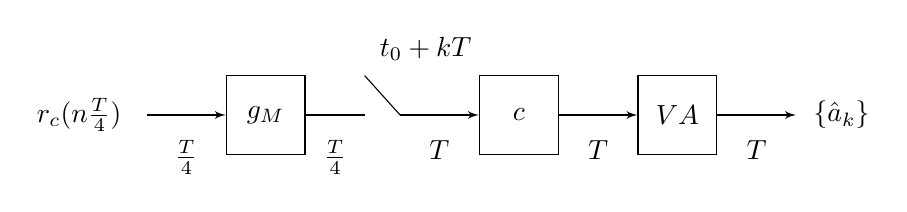
\begin{tikzpicture}[auto,>=latex']
	\tikzstyle{block} = [draw, rectangle, minimum height=1cm, minimum width=1cm]
	
	\node [coordinate, label={[label distance=0.2cm]180:$r_c(n \frac{T}{4})$}] (start) {};
	\node [block, right = 1cm of start] (matchedf){$g_M$};
	\node [coordinate, right = 0.75 cm of matchedf] (c0) {};
	\node [coordinate, above = 0.5 cm of c0, label={[label distance=0.1cm]45:$t_0 + kT$} ] (c1) {};
	
	\node [coordinate, right = 1.2cm of matchedf] (c2) {};
	
	\node [block, right = 1cm of c2] (cfilter){$c$};
	\node [block, right = 1cm of cfilter] (viterbi){$VA$};
	
	\node [coordinate, right = 1cm of viterbi, label={[label distance=0.1cm]0:$\{\hat{a}_k\}$}] (end){};
	
	\draw [->] (start) --node[label={[label distance=0.2cm]270:$\frac{T}{4}$}]{} (matchedf);
	\draw [-] (matchedf) --node[label={[label distance=0.2cm]270:$\frac{T}{4}$}]{} (c0);
	\draw [-] (c1) --node[]{} (c2);
	\draw [->] (c2) --node[label={[label distance=0.2cm]270:$T$}]{} (cfilter);
	\draw [->] (cfilter) --node[label={[label distance=0.2cm]270:$T$}]{} (viterbi);
	\draw [->] (viterbi) --node[label={[label distance=0.2cm]270:$T$}]{} (end);
	
	\end{tikzpicture}
	\caption{Model for the receiver (e).}
	\label{Receiver_e} 
\end{figure}

\clearpage
\subsection*{Receiver f}

\begin{figure}[H]
	\centering
	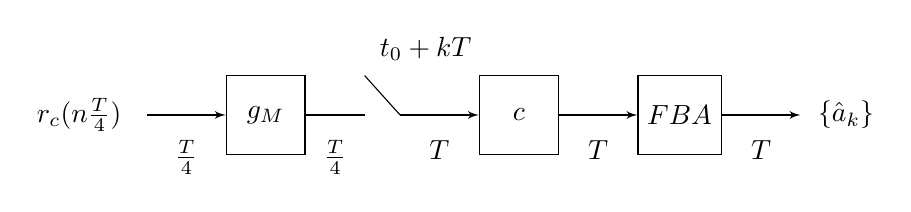
\begin{tikzpicture}[auto,>=latex']
	\tikzstyle{block} = [draw, rectangle, minimum height=1cm, minimum width=1cm]
	
	\node [coordinate, label={[label distance=0.2cm]180:$r_c(n \frac{T}{4})$}] (start) {};
	\node [block, right = 1cm of start] (matchedf){$g_M$};
	\node [coordinate, right = 0.75 cm of matchedf] (c0) {};
	\node [coordinate, above = 0.5 cm of c0, label={[label distance=0.1cm]45:$t_0 + kT$} ] (c1) {};
	
	\node [coordinate, right = 1.2cm of matchedf] (c2) {};
	
	\node [block, right = 1cm of c2] (cfilter){$c$};
	\node [block, right = 1cm of cfilter] (fba){$FBA$};
	
	\node [coordinate, right = 1cm of fba, label={[label distance=0.1cm]0:$\{\hat{a}_k\}$}] (end){};
	
	\draw [->] (start) --node[label={[label distance=0.2cm]270:$\frac{T}{4}$}]{} (matchedf);
	\draw [-] (matchedf) --node[label={[label distance=0.2cm]270:$\frac{T}{4}$}]{} (c0);
	\draw [-] (c1) --node[]{} (c2);
	\draw [->] (c2) --node[label={[label distance=0.2cm]270:$T$}]{} (cfilter);
	\draw [->] (cfilter) --node[label={[label distance=0.2cm]270:$T$}]{} (fba);
	\draw [->] (fba) --node[label={[label distance=0.2cm]270:$T$}]{} (end);
	
	\end{tikzpicture}
	\caption{Model for the receiver (f).}
	\label{Receiver_f} 
\end{figure}

\end{document}